\documentclass[12pt, oneside]{article}
\usepackage[letterpaper, margin=1in, headsep=0.5in]{geometry}
\usepackage[english]{babel}
\usepackage[utf8]{inputenc}
\usepackage{amsmath}
\usepackage{amsfonts}
\usepackage{amssymb}
\usepackage{tikz}
\usetikzlibrary{quotes, angles}
\usepackage{graphicx}
%\usepackage{pgfplots}
%\pgfplotsset{width=10cm,compat=1.9}
%\usepgfplotslibrary{statistics}
%\usepackage{pgfplotstable}
%\usepackage{tkz-fct}
%\usepackage{venndiagram}
\usepackage{multicol}

\usepackage{fancyhdr}
\pagestyle{fancy}
\fancyhf{}
\rhead{\thepage \\Name: \hspace{1.5in}.\\}
\lhead{BECA / Dr. Huson / 11.1 IB Math SL\\* 21 May 2019}

\renewcommand{\headrulewidth}{0pt}

\begin{document}
  \begin{enumerate}


\subsubsection*{Fitting linear models and interpreting correlation}
\item Dr. Huson buys a new plant and measures how tall it is after a number of weeks. Some of his measurements are shown below. Plot the points in the grid below.
  \renewcommand{\arraystretch}{1.6}
    \begin{center}
      \begin{tabular}{|l|r|r|r|r|}
      \hline
      Weeks & 2 & 5 & 7 & 10\\
      \hline
      Height (cm) & 5 & 6 & 8 & 9 \\
      \hline
      \end{tabular}
    \end{center}

\begin{center} %4 quadrant regents grid w T-Chart
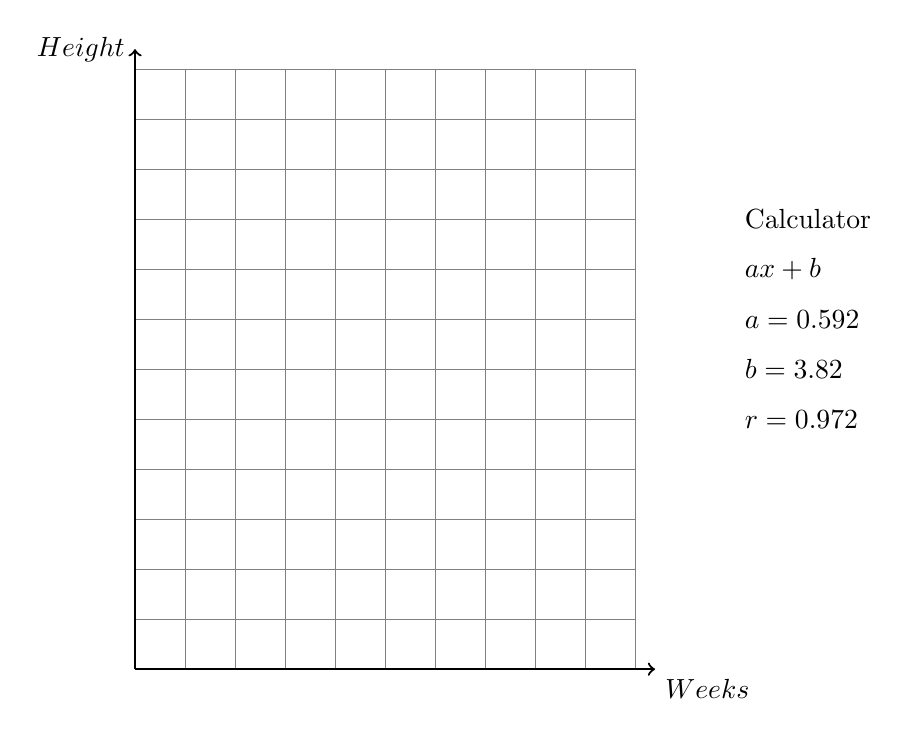
\begin{tikzpicture}[scale=.635]
  \draw [help lines] (0,0) grid (10,12);
  \draw [thick, ->] (0,0) -- (10.4,0) node [below right] {$Weeks$};
  \draw [thick, ->] (0,0)--(0,12.4) node [left] {$Height$};
  \node at (12,9)[right]{Calculator};
  \node at (12,8)[right]{$ax+b$};
  \node at (12,7)[right]{$a=0.592$};
  \node at (12,6)[right]{$b=3.82$};
  \node at (12,5)[right]{$r=0.972$};
\end{tikzpicture}
\end{center}
State, to the \emph{nearest tenth}, the linear regression equation that approximates the height, $y$, of the plants after $x$ weeks.\\[2cm]
Explain what the $y$-intercept means in the context of the problem. \\[3cm]
Explain what the slope means in the context of the problem.
\newpage
\subsubsection*{Simplifying polynomials, standard form}

\item Simplify the expresion $2x + 3(x+5)+4$.\vspace{3cm}
\item Write the expression $3x+2x^2-6x^2+9x+5+3x$ as a polynomial in standard form. \vspace{4cm}

  \item Write the expression $5x+4x^2(2x+7)-6x^2-9x$ as a polynomial in standard form. \vspace{4cm}

  \item Simplify $x^2-3x -4 +2x^2+2x+4$ \vspace{3cm}
  \item Simplify $5(a^2-3a +1) -2(a^2+2a-3)$ \vspace{3cm}


\end{enumerate}
\end{document}
